\section{CMAC}\label{sec:6-10}

基于密码的 MAC——CMAC——是美国国家标准研究所 (NIST) 在 2005 年采用的一个 ECBC 的变体。它基于 John Black 和 Phillip Rogaway 的一个提案,以及岩田哲 (Tetsu Iwata) 和黑泽馨 (Kaoru Kurosawa) 对它的一个扩展。CMAC 在两个方面改进了 ANSI 标准中所使用的 ECBC。首先,CMAC 使用随机化的无前缀编码将无前缀安全的 PRF 转换成安全的 PRF。这种设计省略了 ECBC 中所使用的最终加密步骤。其次,CMAC 使用了一种``双密钥"方法,以避免在输入消息长度是底层 PRF 分组长度的整数倍时需要附加一个假分组的问题。

CMAC 是使用 CBC 无前缀安全 PRF 建立按比特安全的 PRF 的最佳方法。它应该被用于代替所有的 ANSI 方法。在练习 6.14 中,我们表明,CMAC 构造同样适用于级联的场合。

\begin{snote}[CMAC 按比特 PRF。]
CMAC 算法由两个步骤组成。首先,一个子密钥生成算法被用来从 MAC 密钥 $k$ 派生出三个子密钥 $k_0$,$k_1$ 和 $k_2$。然后,这三个子密钥 $k_0$,$k_1$ 和 $k_2$ 被用来计算 MAC。

令 $F$ 是一个定义在 $(\mathcal{K},\mathcal{X},\mathcal{X})$ 上的PRF,其中 $\mathcal{X}=\{0,1\}^n$。NIST 标准使用 AES 作为 PRF $F$。我们在表 \ref{tab:6-1} 详细介绍了 CMAC 签名算法,并用图 \ref{fig:6-8} 给出了直观的展示。当消息长度是分组长度 $n$ 的整数倍时,我们就使用左图所展示的方法,否则就使用右图。该标准允许将最终输出截短到 $w$ 比特,只需要输出最终值 $t$ 的 $w$ 个最高有效比特。
\end{snote}

\begin{table}
	\hspace*{5pt} 输入:密钥 $k\in\mathcal{K}$ 和 $m\in\{0,1\}^*$\\
	\hspace*{26pt} 输出:标签 $t\in\{0,1\}^w$,其中 $w\leq n$

	\vspace{3pt}

	\hspace*{5pt} \underline{设置}:\\
	\hspace*{26pt} 运行一个子密钥生成算法,由 $k\in\mathcal{K}$ 生成子密钥 $k_0,k_1,k_2\in\mathcal{X}$\\
	\hspace*{26pt} 令 $\ell\leftarrow\mathrm{length}(m)$\\
	\hspace*{26pt} 令 $u\leftarrow\mathrm{max}(1,\lceil\ell/n\rceil)$\\
	\hspace*{26pt} 将 $m$ 切分成长为 $n$ 比特的连续分组,使得 $m=a_1\,\Vert\,a_2\,\Vert\,\cdot\,\Vert\,a_{u-1}\,\Vert\,a_u^*$,其中 $a_1,\dots,a_{u-1}\in\{0,1\}^n$\\
	\hspace*{26pt} 如果 $\mathrm{length}(a_u^*)=n$:\\
	\hspace*{50pt} 则令 $a_u=k_1\oplus a_u^*$\\
	\hspace*{50pt} 否则令 $a_u=k_2\oplus(a_u^*\,\Vert\,1\,\Vert\,0^j)$,其中 $j=nu-\ell-1$
	
	\vspace{3pt}
	
	\hspace*{5pt} \underline{CBC}:\\
	\hspace*{26pt} 令 $t\leftarrow0^n$\\
	\hspace*{26pt} 对于 $i=1,\dots,u$:\\
	\hspace*{50pt} 令 $t\leftarrow F(k_0,\;t\oplus a_i)$\\
	\hspace*{26pt} 输出 $t[0\dots w-1]$ \quad\quad\quad\quad\quad // \emph{输出 $t$ 的 $w$ 个最高有效比特}
  \caption{CMAC 签名算法}
  \label{tab:6-1}
\end{table}

\begin{figure}
  \centering
  \subfigure[当$\mathrm{length}(m)$ 是 $n$的正整数倍时]{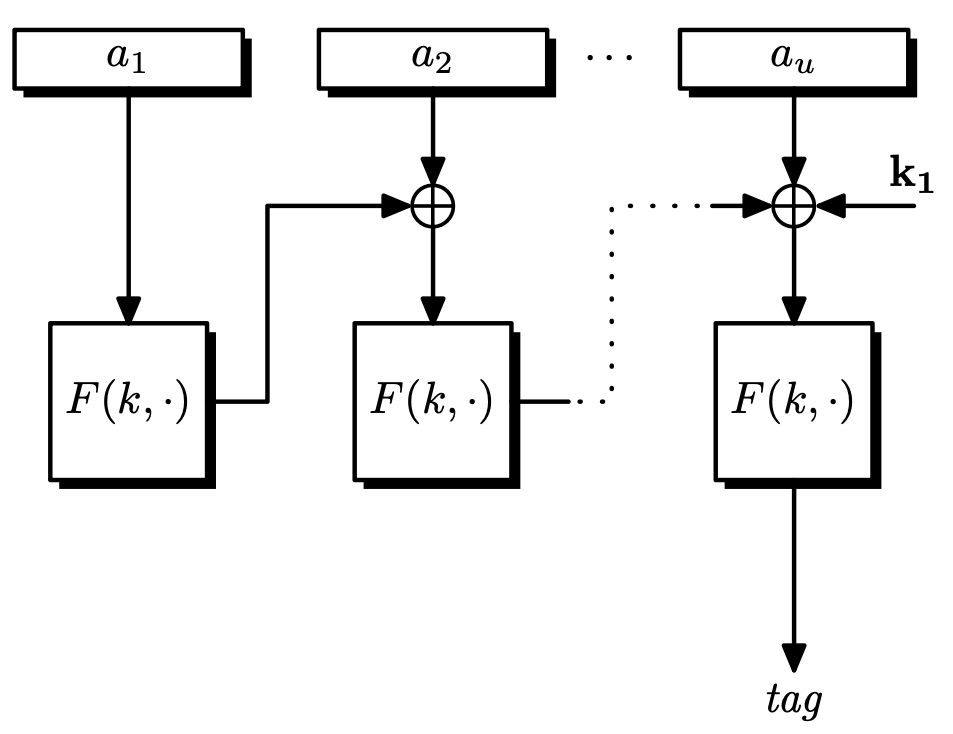
\includegraphics[width=0.43\linewidth]{figures/chapter6/fig8-a.png}}
  \quad\quad\quad
  \subfigure[其他情况]{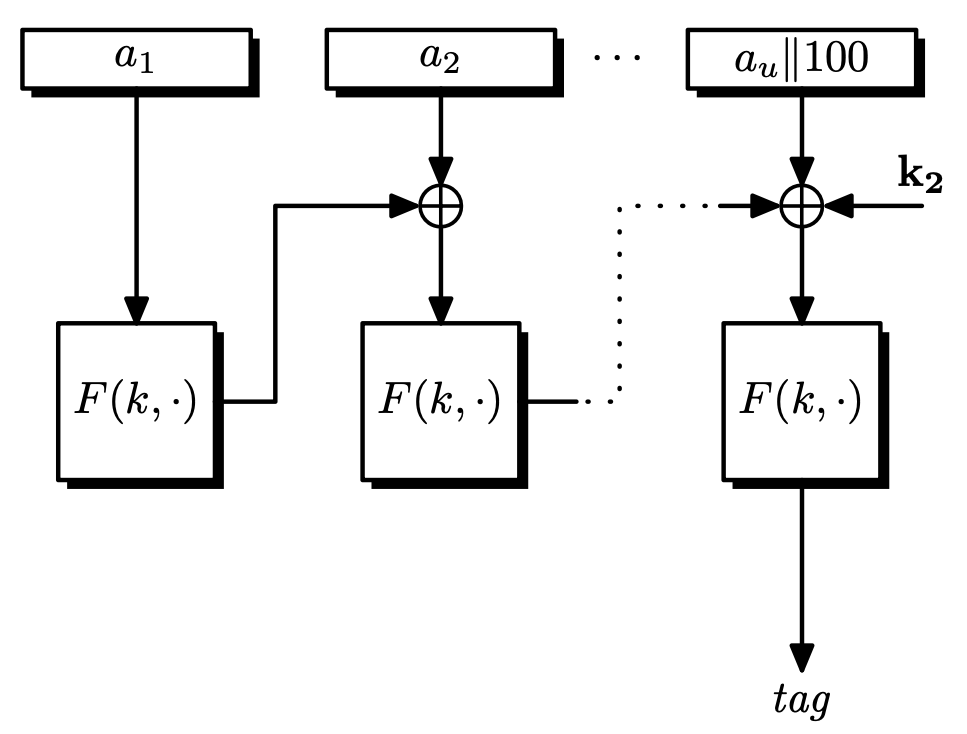
\includegraphics[width=0.43\linewidth]{figures/chapter6/fig8-b.png}}
  \caption{CMAC签名算法}
  \label{fig:6-8}
\end{figure}

\begin{snote}[安全性。]
图 \ref{fig:6-8} 中所描述的 CMAC 算法可以用随机化无前缀编码的范式来分析。实际上,CMAC 使用一个随机化无前缀编码 $rpf:\mathcal{K}\times\mathcal{M}\to\mathcal{X}^{\leq\ell}_{_{>0}}$ 将 CBC 无前缀安全的 PRF 直接转换为\emph{按比特}安全的 PRF,其中 $\mathcal{K}:=\mathcal{X}^2$,$\mathcal{M}:=\{0,1\}^{\leq n\ell}$。编码 $rpf$ 的定义如下:

\vspace{5pt}

\hspace*{5pt} 输入:$m\in\mathcal{M}$ 和 $(k_1,k_2)\in\mathcal{K}^2$

\vspace{3pt}

\hspace*{5pt} 如果 $|m|$ 不是 $n$ 的正整数倍:\\
\hspace*{50pt} 令 $u\leftarrow |m|\;\mathrm{mod}\;n$\\
\hspace*{26pt} 将 $m$ 切分为一连串的比特序列 $a_1,\dots,a_v\in\mathcal{X}$,\\
\hspace*{50pt} 因此,$m=a_1\,\Vert\,\dots\,\Vert\,a_v$ 和 $a_1,\dots,a_{v-1}$ 都是 $n$ 比特的序列\\
\hspace*{26pt} 如果 $|m|$ 是 $n$ 的正整数倍:\\
\hspace*{50pt} 则输出 $\big(a_1,\,\dots,\,a_{v-1},\,(a_v\oplus k_1)\big)$\\
\hspace*{50pt} 否则输出 $\big(a_1,\,\dots,\,a_{v-1},\,((a_v\,\Vert\,1\,\Vert\,0^{n-v-1})\oplus k_2)\big)$

\vspace{5pt}

\noindent
对 $rpf$ 是一个随机性 $2^{-n}$-无前缀编码的论证与 \ref{sec:6-7} 节中的论证类似。因此,CMAC 符合随机性无前缀编码的范式,其安全性可由定理 \ref{theo:6-9} 推出。密钥 $k_1$ 和 $k_2$ 是用于解决长度为 $n$ 的正整数倍的消息和被填充为 $n$ 的正整数倍的消息之间的碰撞的。这对 CMAC $rpf$ 的分析至关重要。
\end{snote}

\begin{snote}[子密钥生成。]
子密钥生成算法使用密钥 $k$ 生成子密钥 $(k_0,k_1,k_2)$。它使用一个固定的掩码序列 $R_n$,取决于 $F$ 的分组长度。比如说,对于 $128$ 比特的分组长度,标准规定 $R_{128}:=0^{120}10000111$。对于一个比特序列 $X$,我们用 $X\ll1$ 表示将 $X$ 最左侧的比特丢弃,并在最右侧添加一个 $0$ 而产生的新比特序列。于是,子密钥生成算法的工作方式如下:

\vspace{5pt}

\hspace*{5pt} 输入:密钥 $k\in\mathcal{K}$\\
\hspace*{26pt} 输出:子密钥 $k_0,k_1,k_2\in\mathcal{K}$

\vspace{3pt}

\hspace*{5pt} 令 $k_0\leftarrow k$\\
\hspace*{26pt} 令 $L\leftarrow F(k,0^n)$\\
\hspace*{1pt} ($1$)
\hspace*{4.5pt} 如果 $\mathrm{msb}(L)=0$,则令 $k_1\leftarrow (L\ll1)$,否则令 $k_1\leftarrow(L\ll1)\oplus R_n$\\
\hspace*{1pt} ($2$)
\hspace*{4.5pt} 如果 $\mathrm{msb}(k_1)=0$,则令 $k_2\leftarrow (k_1\ll1)$,否则令 $k_2\leftarrow(k_1\ll1)\oplus R_n$\\
\hspace*{26pt} 输出 $k_0,k_1,k_2$

\vspace{5pt}

\noindent
其中,$\mathrm{msb}(L)$ 指的是 $L$ 的最高有效比特。标有 ($1$) 和($2$) 的两行看起来有点神秘,但它们实际上只是在有限域 $\mathrm{GF}(2^n)$ 中(分别)用 $L$ 乘以 $X$ 和 $X^2$。在这里,我们将 $\mathrm{GF}(2^n)$ 中的元素视为用 $\mathbb{F}_2[X]$ 中的多项式模一个固定多项式 $g(X)$ 后的结果。对于 $128$ 比特的分组长度,对应于 $R_{128}$ 的定义多项式$g(X)$ 是 $g(X):=X^{128}+X^7+X^2+X+1$。练习 6.16 探讨了子密钥生成的一些不安全的变体。

子密钥生成算法输出的三个密钥 $(k_0,k_1,k_2)$ 可以被用来认证多条消息。因此,它的运行时间可以分摊到多条消息之中。

密钥 $k_0$,$k_1$ 和 $k_2 $ 显然不是独立的。如果它们是独立的,或者如果它们被派生成相互独立的,比如对于常量 $\alpha_0$,$\alpha_1$ 和 $\alpha_2$,令 $k_i:=F(k,\alpha_i)$,CMAC 的安全性就可以直接由这里的论证和我们的通用框架得到。然而,借由更复杂的分析,我们也能证明 CMAC 事实上确实是安全的。
\end{snote}